\chapter{Fundamentação Teórica}
\label{cap:fundamentacao-teorica}

Esta seção apresenta os fundamentos teóricos relacionados às redes
neurais artificiais (RNA) e algumas arquiteturas dessas redes. Primeiramente na seção 2.1 discorreremos à cerca das RNA em seguida na seção 2.2 falaremos sobre a rede \textit{Multilayer Perceptron} (MLP), depois na seção 2.3 falaremos sobre a \textit{Radial Basis Function}(RBF), na seção 2.4 sobre \textit{Adaptive Resonance Theory}(ART), depois na seção 2.5 sobre a rede \textit{Kohonen} e finalmente na seção 2.6 concluiremos o capítulo.

\section{Redes Neurais}
\label{sec:redes-neurais}

As redes neurais artificias(RNA) são inspirados nas redes neurais biológicas, pode-se definir como um conjunto de unidades de processamento na qual tem a capacidade de adquirir e processar conhecimento \cite{silva2010redes}.Em RNA os neurônios artificiais possuem ligações através de sinapses artificias que são na realidades um conjunto de vetores ou matrizes de pesos sinápticos.








\section{MLP}
\label{sec:multilayer-perceptron}

A MLP é uma rede neural de treinamento supervisionado e tem como uma das suas características a utilização de no mínimo uma camada intermediária de neurônios entre a camada de entrada e a camada de saída, entretanto, este modelo é constituído de múltiplas camadas de neurônios, onde essas camadas são interconectadas às camadas posteriores em direção a camada de saída \cite{gardner1998artificial} .


	\begin{figure}[t]
	\centering
	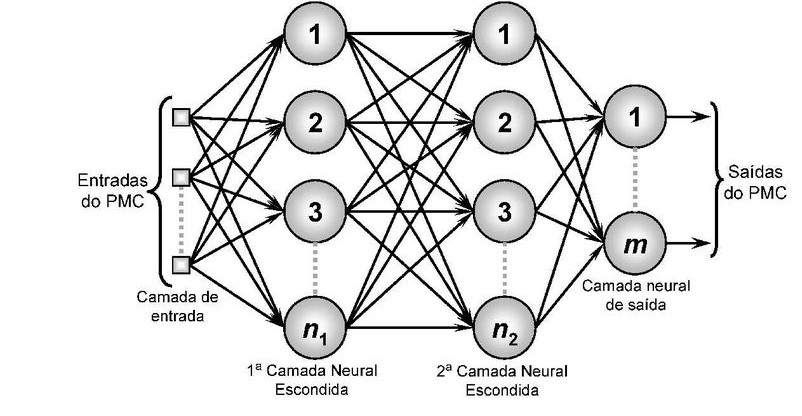
\includegraphics[width=8cm]{figuras/mlp.jpg}
	\caption{Ilustração da MLP}
	\fonte{\cite{silva2010redes}}
\end{figure}

As MLP tem como característica o fato de ser uma das mais versáteis redes com aplicação em diversas áreas de conhecimento entre essas áreas podemos destacar:

\begin{itemize}
	\item Aproximação universal de funções;
	\item Reconhecimento de funções
	\item Previsão de séries temporais	
\end{itemize}




\subsection{Processo de treinamento da MLP}
\label{sub:processo-de-treinamento-da-mlp}


O perceptron Multicamadas utiliza um processo de treinamento chamado \textit{backpropagation} que é dividido em duas fases, sendo a primeira a \textit{forward} (propagação adiante), onde o conjunto de amostras de treinamento são inseridas nas entradas da rede e são propagadas camada a camada até a produção da saída respectiva.

A segunda fase é chamada de \textit{backward} (propagação reversa) onde os pesos sinápticos e limiares são ajustados durante o processo. As aplicações sucessivas de \textit{backward} fazem com que os pesos sinápticos e os limiares sejam ajustados automaticamente em cada iteração, implicando-se gradativa diminuição da soma dos erros produzidos pelas respostas da rede frente aquelas desejadas.


\section{Radial Basis Function}
\label{sec:radial-basis-function}

\section{Adaptive Resonance Theory}
\label{sec:adaptive-resonance-theory}


\section{Kohonen}
\label{sec:kohonen}


\section{Conclusão}
\label{sec:conclusão}
